\chapter{Data Evaluation}\label{chap:de}
This chapter is a consequence of the conducted and normalized measurements performed using a single-antenna \acs{DUT} and a multi-antenna \acs{DUT}. Each test is run for many times in-order to assess the \acf{MU}. 

\section{Measurement Analysis}
This section is sub-divided into two other sections: first when the \acs{DUT} behaves as a transmitter and second when \acs{DUT} is a receiver. This sections also explains the reasons for using the fritz box as a companion device for \acs{PSD} measurement and for using some different spectrum analyzer settings from the settings mentioned by the standard.


\subsection{\acs{DUT} functions as transmitter}
The procedure for the \acf{OBW} measurement and \acf{PSD} are explained in detail in chapter \ref{chap:test}. Figure \ref{fig:nt} depicts the measurement when the \acs{DUT} acts like a transmitter and sends echo packets. The spectrum analyzer saves the traces so that we can measure the bandwidth and the \acf{PSD} of the signal from the \acs{DUT}. When using a golden device or fritz box (section \ref{sec:golden}) as a companion device, data is transmitted and not just \acs{ICMP} packets.


\begin{figure}[H]
\centering
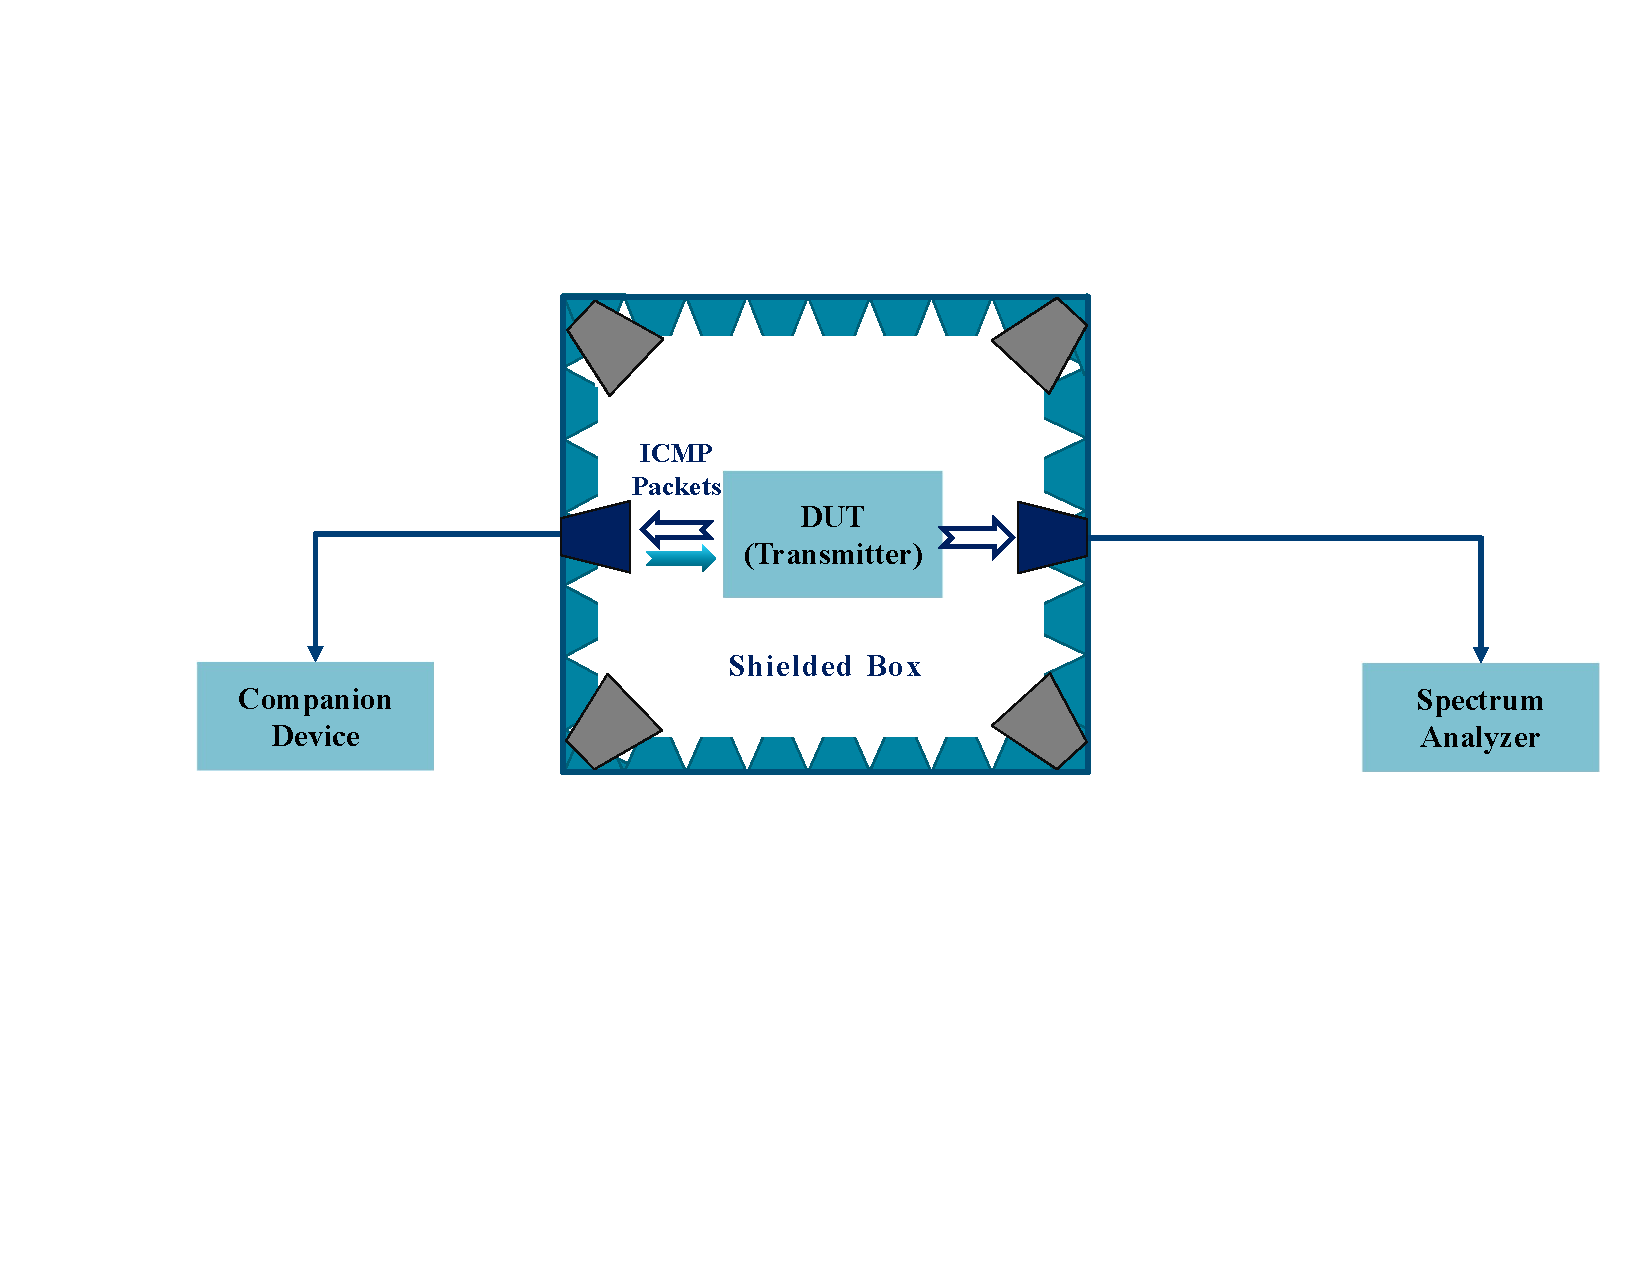
\includegraphics[scale = 0.46]{normalized_dut_transmitter.pdf}
\vspace{-0.5cm}
\caption{Normalized measurement when the \acs{DUT} functions as a transmitter}
\label{fig:nt} 
\end{figure}

Attenuation in the signal analyzer settings is kept to 10 dB and the pre-amplification is switched-off for conducted measurements because of the need of the signal to have a  high dynamic-range, i.e. to make sure that the power envelope is sufficiently above the noise floor of the analyser and to avoid the noise signals left and right from the power envelope being taken into account by this measurement. But, during radiated measurements, the pre-amplification is switched-on and the attenuation is brought down to 0 dB. This is because if the same conducted measurement settings are applied to radiated measurements, the dynamic-range and the noise floor of the signal is low which therefore increases the bandwidth of the signal (Figure \ref{fig:o}). 

\begin{figure}[H]
  \centering
  \subfigure[Bandwidth measurement with proper analyzer settings]{\includegraphics[width=0.49\textwidth]{OCBW_OTA_ATT0.png}} 
  \centering
  \subfigure[Low dynamic range of the system causing increase in bandwidth]{\includegraphics[width=0.49\textwidth]{{OCBW_OTA_ATT10.png}}} 
\caption{Increase in bandwidth of the signal due to low dynamic range}
\label{fig:o}
\end{figure}

The settings for the analyzer mentioned above also applies to \acf{PSD} measurement. In-addition to that, after running the \acs{PSD} measurement only for few times, there is a difference in the result every single time. This can be clearly seen from Figure \ref{fig:psdpsd}. The maximum value is 8.64 dBm and minimum is 7.12 dBm and hence there difference between the two is around 1 dBm which does not look very good. Therefore fritz box is used as a companion device for this measurement instead of the connectivity tester.
\begin{figure}[H]
\centering
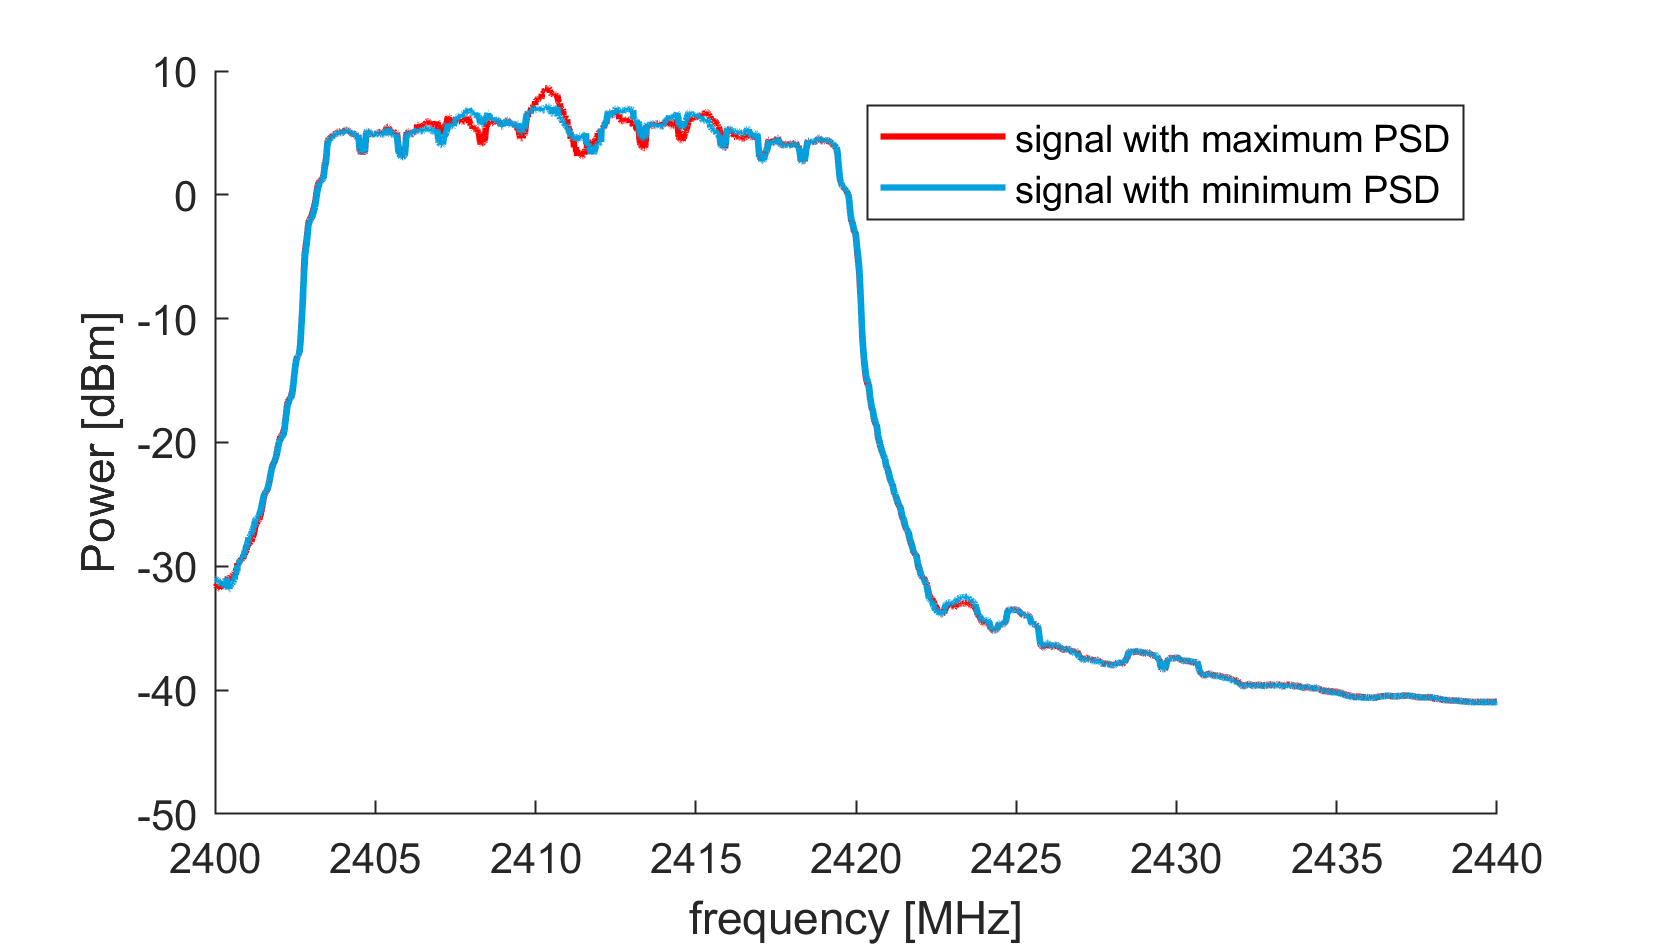
\includegraphics[scale = 0.65]{PSD_trace_differnce.png}
\caption{\acf{MU} in the \acs{PSD} measurement caused due to low duty cycle of the signal}
\label{fig:psdpsd} 
\end{figure}



\subsection{\acs{DUT} functions as receiver}
Figure \ref{fig:nr} pictures the \acs{DUT} as a receiver. This is achieved by using \acf{PER} measurement (section \ref{sec:rxmeas}).

\begin{figure}[H]
\centering
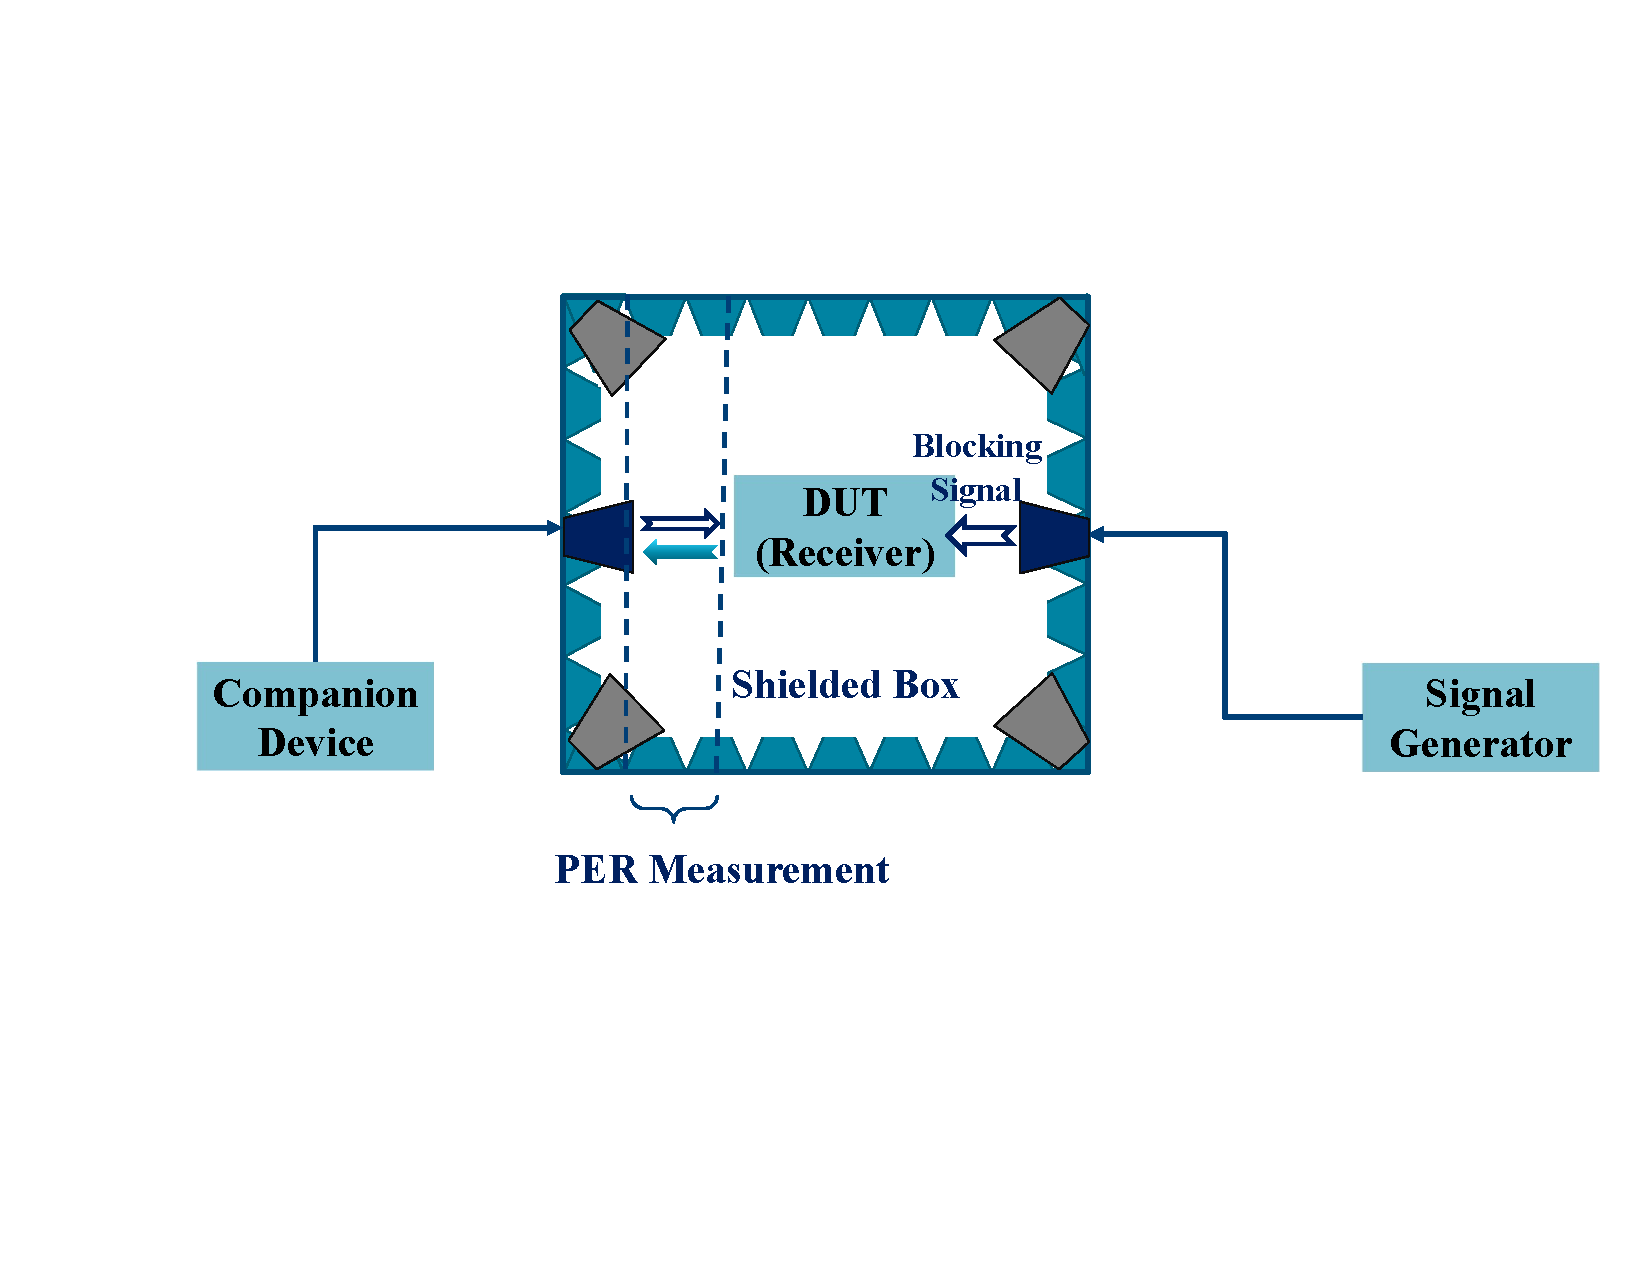
\includegraphics[scale = 0.46]{normalized_dut_receiver.pdf}
\vspace{-1.1cm}
\caption{Normalized measurement when the \acs{DUT} functions as a receiver}
\label{fig:nr} 
\end{figure}

The spectrum analyzer shows the DUT signal and the blocking signal. It can be seen that the signal from the blocker is not very far from the in-band frequency of the \acs{DUT}.
\begin{figure}[H]
\centering
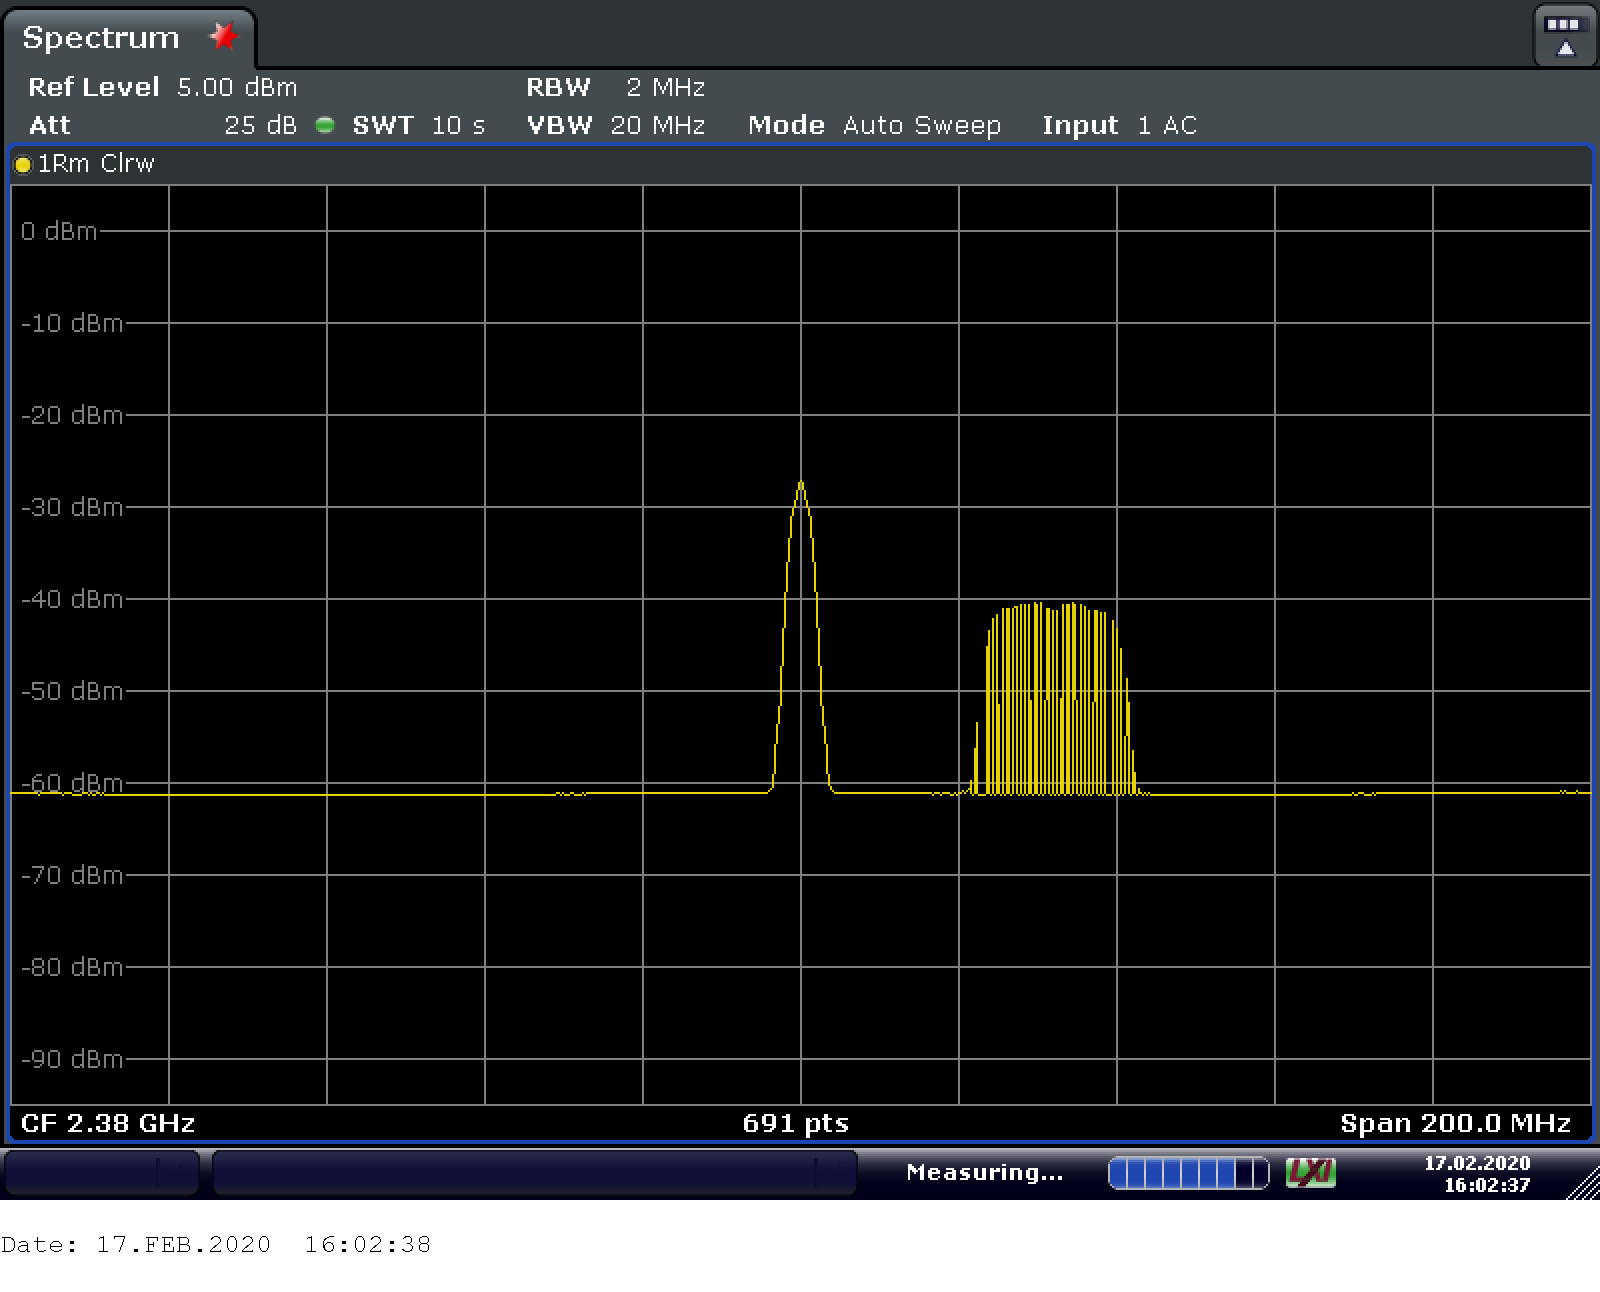
\includegraphics[scale = 0.24]{analyzer_rx.PNG}
\caption{Trace on the spectrum analyzer \acs{GUI}}
\label{fig:ax} 
\end{figure}



\section{\acf{MU}}
The test was run for 300 times and the result using signal antenna DUT and multi antenna DUT are shown as follows. The figure in the left shows result from single antenna DUT and the one in the right is result from multi antenna DUT.
From the plots it is obvious that the measurement uncertainty is higher when using a DUT with multiple antennas. Is this expected? And is this really due to multiple antennas or something else (e.g. lower output power)?




The receiver blocking test is run 21 times and the histogram depicts the occurrence of the blocker level which results in 10\% PER at each frequency. The calculation of mean is done by converting the power level from dBm scale to linear scale because it is physically correct to use mean from the linear scale. The standard deviation is calculated by using the power values in dBm scale. 